\documentclass{article}

\usepackage[printqrbox=false,printhint=false,printanswer=true,printmarkingguide=false,printdraftpaper=false]{unswalgos}

\usepackage{tikz}
\usetikzlibrary{patterns}
\usetikzlibrary{shapes,fit}
\usepackage{tkz-fct}
\usepackage{wrapfig}
\usepackage{subfig}

\usepackage{mathtools}
\usepackage{amssymb}
\usepackage{booktabs,multicol,multirow}
\usepackage{wasysym}
\usepackage{tcolorbox}

\DeclareMathOperator*{\argmax}{arg\,max}
\DeclareMathOperator*{\argmin}{arg\,min}
\DeclareMathOperator{\NAND}{NAND}
\DeclareMathOperator{\AND}{AND}
\DeclareMathOperator{\OR}{OR}
\DeclareMathOperator{\NOT}{NOT}

\usepackage{xspace}

\fancyfoot[L]{\leftmark}
\fancyfoot[R]{\rightmark}

\usepackage{graphicx}
\usepackage{float}
\usepackage{subfigure}

\usepackage{framed}
% This enables new paragraphs without indentation
\usepackage[parfill]{parskip}

\newcommand{\sem}{22T2}
\newcommand{\semester}{Term 2, 2022}
\SubjectNo{COMP3151}
\newcommand{\taskname}{Homework 6}
\Institution{Jinghan Wang, z5286124} % Replace this with your name and zID


\begin{document}

\setcounter{question}{0}

\begin{Question} [\large\textbf {Non-compositional Verification{[6 marks]}}]
    Here is a three process message passing system presented as a transition diagram of three processes $P1$, $P2$, and $P3$.
\begin{figure}[H]
    \centering 
    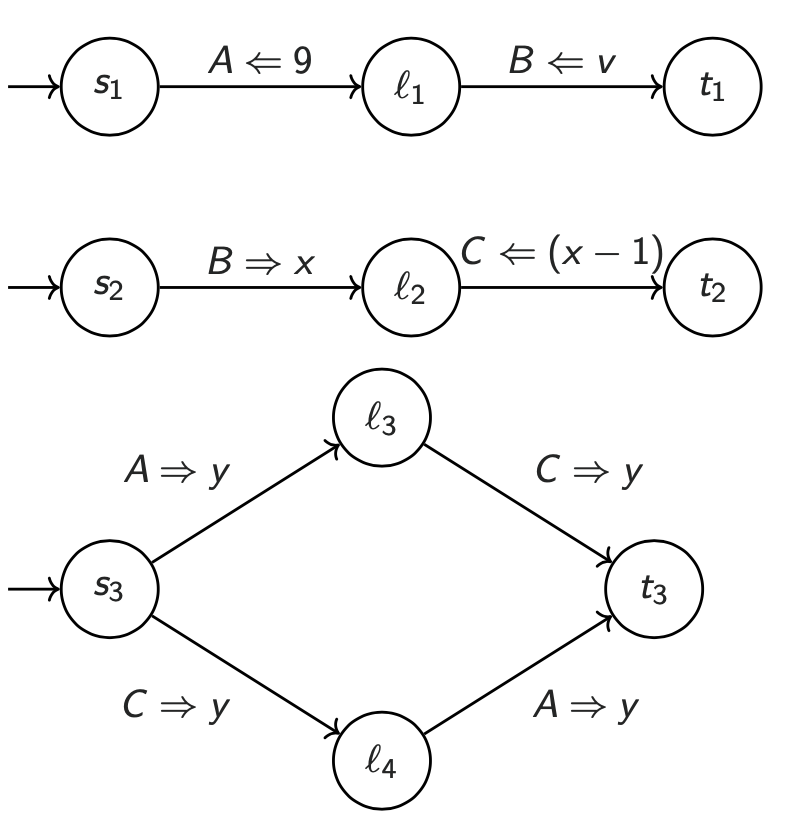
\includegraphics[width=0.75\textwidth]{DV_demand1}
\end{figure}
Prove using the Levin and Gries or AFR methods that the following Hoare triple holds:
\begin{center}
    $\{True\}\ P1\ \|\ P2\ \|\ P3\ \{y=v-1\}$
\end{center}
You don't need to explicitly discharge your proof obligations; instead, it suffices to give your assertion networks, your extra auxiliary variable wrangling, and (if using AFR) your communication invariant.
    
\begin{answer}
    Answer:
    \begin{figure}[H]
        \centering 
        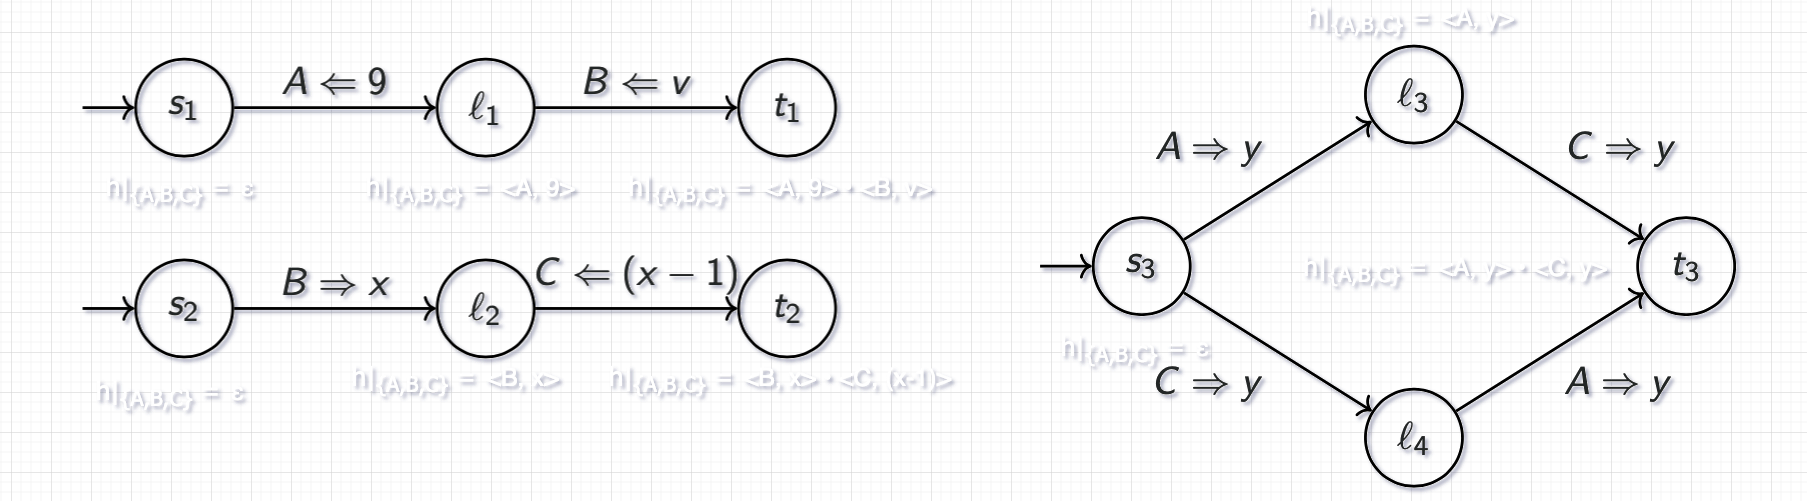
\includegraphics[width=\textwidth]{DV_demand3}
    \end{figure}
\end{answer}
\clearpage
\begin{answer}
    Answer:
    \begin{quote}
        For the three process passing system, there are three channel $(A, B, C)$ to pass the message.
            \begin{itemize}
                \item [$\bullet$] For channel $A$, $A \Leftarrow  9\ (s_1 \rightarrow l_1)$, $A \Rightarrow y\ (s_3 \rightarrow l_3)$, $A \Rightarrow y\ (l_4 \rightarrow t_3)$
                \item [$\bullet$] For channel $B$, $B \Leftarrow v\ (l_1 \rightarrow t_1)$, $B \Rightarrow x\ (s_2 \rightarrow l_2)$
                \item [$\bullet$] For channel $C$, $C \Leftarrow (x-1)\ (l_2 \rightarrow t_2)$, $C \Rightarrow y\ (l_3 \rightarrow t_3)$, $C \Rightarrow y\ (s_3 \rightarrow l_4)$
            \end{itemize}
        As the channel is not Asynchronous channel, a sender input must match a receiver output. \\
        For channel $A$ and $C$, there is a input and two output. for channel; For channel $B$, there is one input and one output. The premise of finishing the message passing in channel $B$ is that complete the $A \Leftarrow 9$ in $P_1$. In $P_3$, it exists two output, however, $A \Rightarrow y\ (l_4 \rightarrow t_3)$ has a premise of $C \Rightarrow y$, the input of channel $C$ is after the $B \Rightarrow x$ in $P_2$, therefore, this way will blocked. The other passing in C $(s_3\rightarrowl_3\rightarrowt_3)$ is suitable of the topic.\\
    \end{quote}

Proof:
    \begin{quote}
        \textbf{Basic diagram rule gives us:}
        \begin{center}
            $\{h|_{\{A, B, C\}} = \varepsilon\}\ P_1\ \{h|_{\{A, B, C\}} =\ <A, 9>\cdot <B, v>\} $\ \ \ \ \ \ \ \ \ (1)\vspace{1ex}\\
            $\{h|_{\{A, B, C\}} = \varepsilon\}\ P_2\ \{h|_{\{A, B, C\}} =\ <B, x>\cdot <C, (x-1)>\} $  (2)\vspace{1ex}\\
            $\{h|_{\{A, B, C\}} = \varepsilon\}\ P_3\ \{h|_{\{A, B, C\}} =\ <A, y>\cdot <C, y>\} $\ \ \ \ \ \ \ \ \ (3)\\
        \end{center}
        \textbf{Apply the parallel composition rule.}\vspace{1ex}\\
        $\{h|_{\{A, B, C\}} = \varepsilon\ \land\ h|_{\{A, B, C\}} = \varepsilon\ \land\ h|_{\{A, B, C\}} = \varepsilon\}\ P_1\ \|\ P_2\ \|\ P_3\ \{ h|_{\{A, B, C\}} =$\vspace{1ex}\\$<A, 9>\cdot <B, v>\ \land\  h|_{\{A, B, C\}} =\ <B, x>\cdot <C, (x-1)>\ \land\ h|_{\{A, B, C\}}$\vspace{1ex}\\$ =\ <A, y>\cdot <C, y>\}$ (4)\vspace{1ex}\\
        \textbf{According to the topic, $y$ is assigned to channel $A$'s output as $9$, and then to channel $C$'s output as $(x-1)$.}\\
        \textbf{Using the rule of consequence with (4) we get:}
        \begin{center}
            $\{h|_{\{A, B, C\}} = \varepsilon\}\ P_1\ \|\ P_2\ \|\ P_3\ \{ x = v \land y = (x-1)\}$ (5)\\
        \end{center}
        \textbf{As $x=v, y=(x-1) \rightarrow y = (v-1)$:}
        \begin{center}
            $\{h|_{\{A, B, C\}} = \varepsilon\}\ P_1\ \|\ P_2\ \|\ P_3\ \{ y = (v-1)\}$ (6)\\
        \end{center}
        \textbf{Using the rule of consequence:}
        \begin{center}
            $\{True \land h|_{\{A, B, C\}} = \varepsilon\}\ P_1\ \|\ P_2\ \|\ P_3\ \{ y = (v-1)\}$ (7)\\
        \end{center}
        \textbf{Using the initialization rule:}
        \begin{center}
            $\{True\}\ P_1\ \|\ P_2\ \|\ P_3\ \{ y = (v-1)\}$ (8)\\
        \end{center}
        Therefore, the result is $\{True\}\ P_1\ \|\ P_2\ \|\ P_3\ \{ y = (v-1)\}$ \\
    \end{quote}
\end{answer}
\end{Question}

\clearpage
\setcounter{question}{1}

\begin{Question} [\large\textbf {Termination{[6 marks]}}]
    Consider the following program:
\begin{figure}[H]
    \centering 
    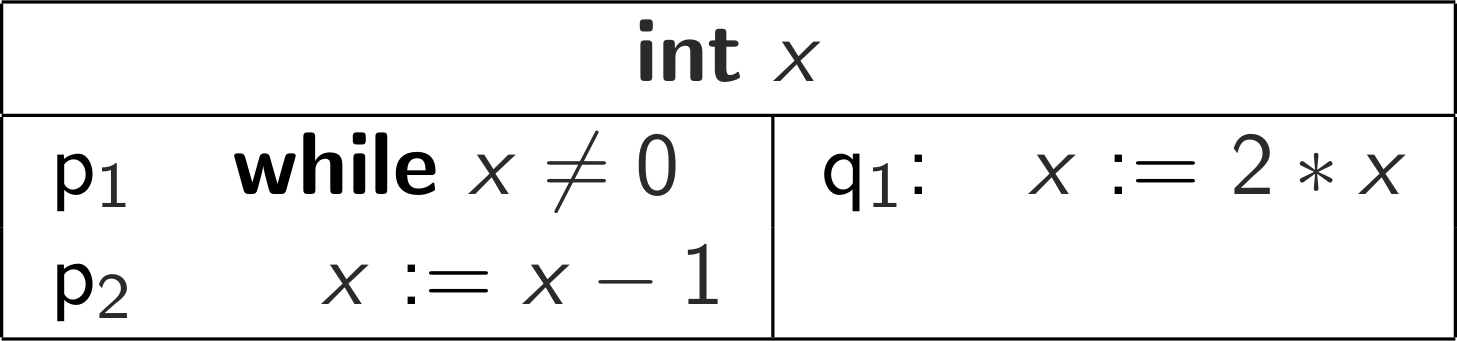
\includegraphics[width=0.9\textwidth]{DV_demand2}
\end{figure}

\begin{Subquestion}
    Use the local method to prove $x\geq0$ -convergence for this program. You'll need exit locations for $p$ and $q$ (not shown in the above pseudocode). You don't need to explicitly discharge your proof obligations; specifying your assertion networks, your wellfounded set, and your ranking functions is sufficient.
    
\begin{answer}
    Answer:
    \begin{quote}
        \begin{figure}[H]
            \centering 
            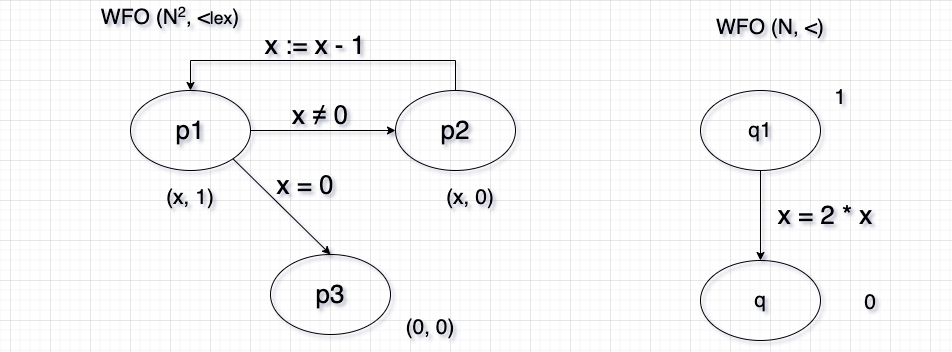
\includegraphics[width=0.9\textwidth]{DV_demand4}
        \end{figure}
        Assertion networks: $\{x\geq 0 \}\ p\ \|\ q\ \{x = 0\}$\\
        ranking:\\
        p:\\
        transition $p1\stackrel{x\neq0}{\longrightarrow}p2$:\ \ \ \ \ $\models (x, 1)\ >_{lex}\ (x, 0)\ \land\ (0, 1)\ >_{lex}\ (0,0)$ \vspace{1em}\\
        transition $p2\stackrel{x:=x-1}{\longrightarrow}p1$:\ \ \ \ \ $\models x \neq 0 \Rightarrow x > x - 1 \geq 0$ \vspace{1em}\\
        transition $p1\stackrel{x=0}{\longrightarrow}p3$:\ \ \ \ \ $\models (0, 1) >_{lex} (0, 0) $ \\\\
        q:\\
        transition $q1\stackrel{x:=x*2}{\longrightarrow}q2$:\ \ \ \ \ $\models 1>0$ \vspace{1em}\\

    \end{quote}
\end{answer}
\end{Subquestion}

\clearpage
\begin{Subquestion}
    Is this program $\top$ -convergent? Briefly motivate your answer.
    
\begin{answer}
    Answer:
    \begin{quote}
        No, for this program, when $x < 0$, the $x$ will decrease forever and never reach the $x=0$ to stop. When $x > 0$, the program, $p$ only minus 1, $q$ will double the value of $x$, it is difficulty to reach the purpose. Therefore, it is not $\top$ -convergent.\\
    \end{quote}
\end{answer}
\end{Subquestion}

\begin{Subquestion}
    Is this program $\bot$ -convergent? Briefly motivate your answer.

\begin{answer}
    Answer:
    \begin{quote}
        Yes, although it is difficulty to reach the purpose, when the initial state is satisfied, the purpose can be achieved. Therefore, it iss $\bot$ -convergent.\\
    \end{quote}
\end{answer}
\end{Subquestion}


\end{Question}
\end{document}